\subsubsection{09.01.15}
\begin{enumerate}
	
	\item Time of beginning and ending of meeting: 15:30 - 21:30.
	
	\item Purposes of meeting: 
	\begin{enumerate}
		
		\item To replace broken slat.
		
		\item To test the programme of control robot when all motors works.
		
		\item To make and install plate that will connect shaft of servo with the axis with driven gear.
		
	\end{enumerate}

	\item Work that has been done:
	\begin{enumerate}
		
		\item Strenghening plate was made and installed on MOB.
				\begin{figure}[H]
					\begin{minipage}[h]{0.2\linewidth}
						\center  
					\end{minipage}
					\begin{minipage}[h]{0.6\linewidth}
						\center{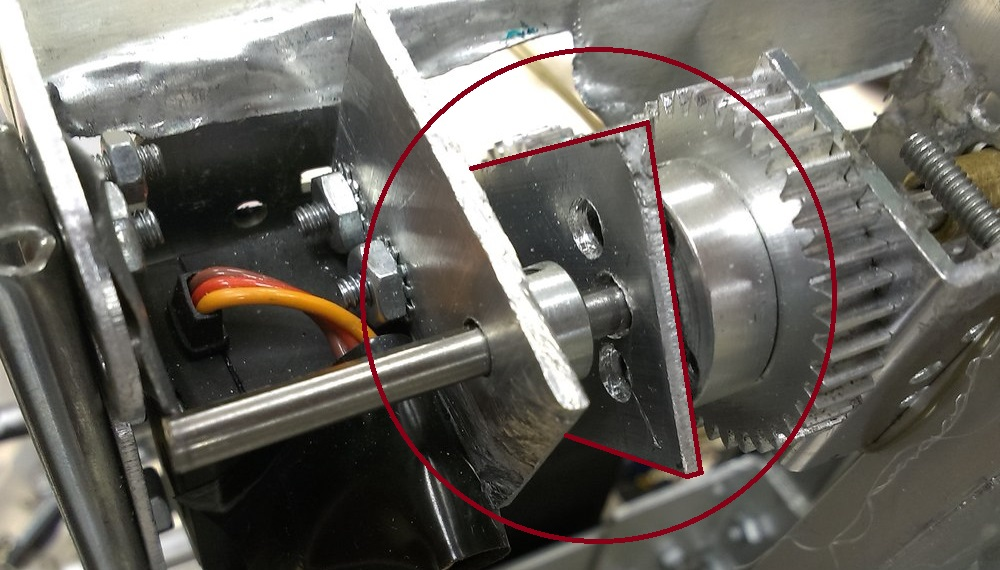
\includegraphics[scale=0.2]{days/10.01.15/images/01}}
						\caption{Strenghening plate}
					\end{minipage}
				\end{figure}
		
		\item Broken slat was replaced. Now we also has another one spare slat 30cm because furniture slats solds in pairs.
		
        \item It was decided to make the gutter that will fix on the top pair of slat by galvanized steel with thickness 0.5mm. The balls will roll from the overturned bucket to the goal. It was decided to make drawing of the gutter and then make it.
        
        \item We couldn't test the programme of control robot because all batteries discharged.
        
	\end{enumerate}
	
	\item Results:
	\begin{enumerate}
		
		\item Broken slat was replaced.
        
        \item The programme of control robot wasn't tested.
		
	\end{enumerate}
	
	\item Tasks for the next meetings:
	\begin{enumerate}
		
		\item To make the drawing of the gutter and make it.
		
        \item To test the programme of control robot.
			
	\end{enumerate}
\end{enumerate}
\fillpage
